\documentclass[12pt]{article}
\usepackage{color}
\usepackage{cite}
\usepackage{geometry}                % See geometry.pdf to learn the layout options. There are lots.
%\usepackage{pdflscape}        %single page landscape
                                %mode \begin{landscape} \end{landscape}
\geometry{letterpaper}                   % ... or a4paper or a5paper or ... 
%\usepackage[parfill]{parskip}    % Activate to begin paragraphs with an empty line rather than an indent
\usepackage{graphicx}
\usepackage{amssymb}
\usepackage{Sweave}
\newcommand{\etal}{\textit{et al.}}
\usepackage{hyperref}  %\hyperref[label_name]{''link text''}
                       %\hyperlink{label}{anchor caption}
                       %\hypertarget{label}{link caption}
\linespread{1.5}

\title{Sunset Crater Rock Lichen Community Composition}
\author{M.K. Lau}
%\date{}                                           % Activate to display a given date or no date

\begin{document}
\maketitle



\section{Questions for Co-Authors}
\begin{enumerate}
\item Were all measurments a part of the same quadrat? 
\item I.E., are lichen/bryophyte measurements ablsolute or a proportion of available
  habitat?
\item Rikke and Cameron, how were the lichen/bryophyte measurements
  done?
\item Richard, how were the plant and light measurements done?
\end{enumerate}

\section{Things to Do}

\begin{itemize}
\item Check Resistance vs Susceptible in barplots
\item Chekc on bird preference
\item Compile trait data from database
\item Check on co-occurrence
\item Do indicator species sems or summed species sems
\item multiple resgresion for variables on community
\end{itemize}


\section{Do rock lichen communities respond to phenotypic variation in
a foundation species?}

\subsection{Load and Pre-Process Data}

\begin{Schunk}
\begin{Sinput}
> key <- read.csv('/Users/Aeolus/Documents/Active_Projects/Sunset_Crater_Lichens/data/key.csv')
> x <- read.csv('/Users/Aeolus/Documents/Active_Projects/Sunset_Crater_Lichens/data/spp_env_combined.csv')
>                                         #remove dead
> x <- x[x$Live.Dead == 1,]
> com <- x[,((1:ncol(x))[colnames(x) == 'Acacon']):((1:ncol(x))[colnames(x) == 'Xanele'])]
> env <- x[,1:12]
>                                         #remove N and S light
> env <- env[,-10:-11]
>                                         #flip R and 
> ## env$Moth[env$Moth==0] <- 2
> ## env$Moth[env$Moth==1] <- 0
> ## env$Moth[env$Moth==2] <- 1
>                                         #fix colnames
> colnames(env) <- sub('\\.\\.','',colnames(env))
> colnames(env)
\end{Sinput}
\begin{Soutput}
 [1] "Tree.pairs"    "Moth"          "Live.Dead"     "Litter"       
 [5] "Big.rocks"     "Small.rocks"   "Shrubs"        "Grass"        
 [9] "Branches"      "Light.average"
\end{Soutput}
\begin{Sinput}
> 
\end{Sinput}
\end{Schunk}

\subsection{Analysis of Moth Affects on "Env" Variables}

%% <<>>=

%% library(vegan)
%% library(mvabund)
%% library(tweedie)
%% library(statmod)
%% library(xtable)
%%                                         #the response of light
%% env. <- env[,c(4:10)]
%% env. <- apply(env.,2,sqrt)
%% mva.env <- mvabund(env.)
%% fit.env <- manyglm(mva.env~env$Moth:env$Tree.pairs,family='gaussian')
%% summary(fit.env,p.uni='unadjusted')
%% p.adjust(summary(fit.env,p.uni='unadjusted')$uni.p[,2],method='fdr')

%% @ 

\begin{Schunk}
\begin{Sinput}
> shapiro.test(fit.env$residuals)
\end{Sinput}
\begin{Soutput}
	Shapiro-Wilk normality test

data:  fit.env$residuals 
W = 0.9019, p-value = 8.339e-16
\end{Soutput}
\begin{Sinput}
> par(mfrow=c(1,2))
> plot(fit.env$residuals~fit.env$fitted)
> abline(h=0)
> hist(fit.env$residuals)
> 
\end{Sinput}
\end{Schunk}
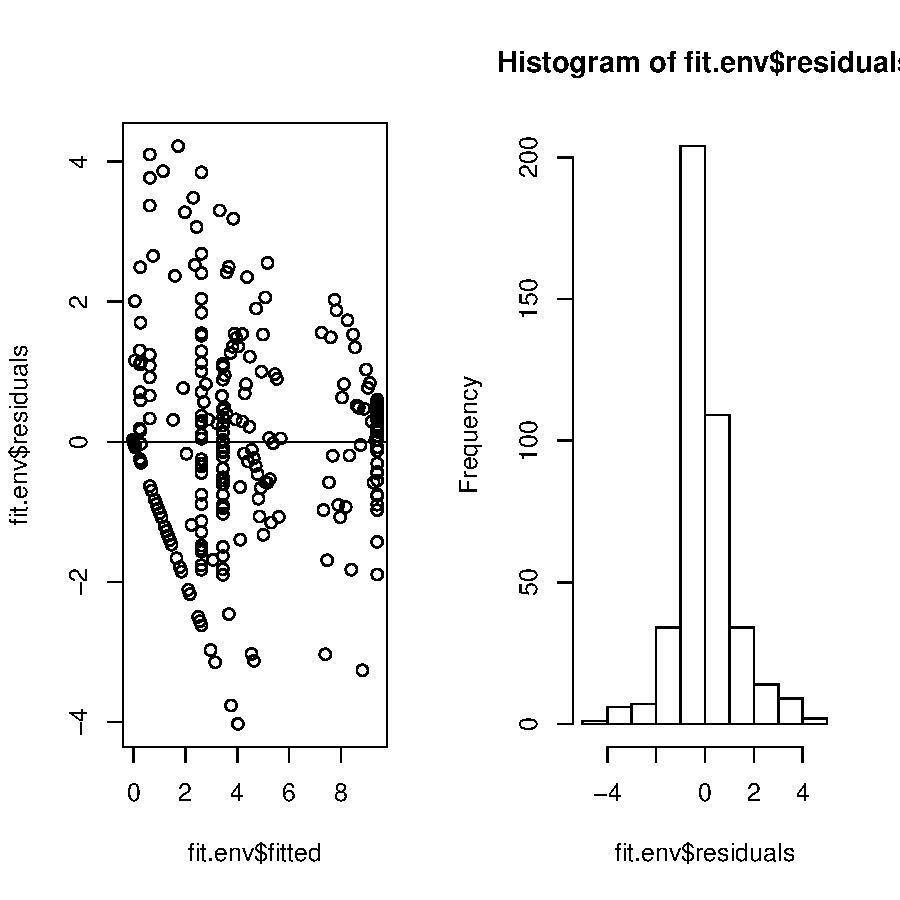
\includegraphics{SCRL-002}

\begin{Schunk}
\begin{Sinput}
> library(gplots)
> par(mfrow=c(2,4))
> for (i in 4:ncol(env)){
+   mu <- tapply(env[,i],env$Moth,mean)
+   se <- tapply(env[,i],env$Moth,function(x)sd(x)/sqrt(length(x)))
+   x.names <- unique(env$Moth)
+   x.names[x.names==1] <- 'R'
+   x.names[x.names==0] <- 'S'
+   barplot2(mu,plot.ci=TRUE,ci.l=mu-se,ci.u=mu+se,ylab=colnames(env)[i],names=x.names)
+ }
> 
\end{Sinput}
\end{Schunk}
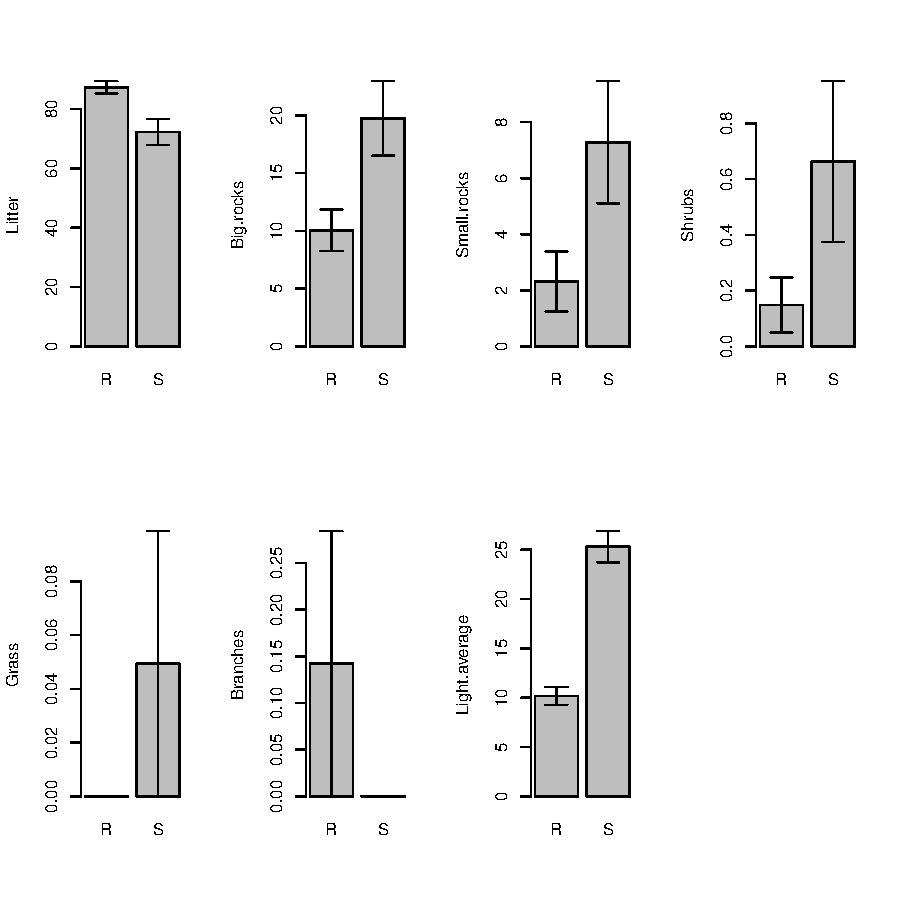
\includegraphics{SCRL-003}


\begin{Schunk}
\begin{Sinput}
>   pairs(env[,c(-2:-3,-8:-11)],lower.panel=panel.cor)
> 
\end{Sinput}
\end{Schunk}
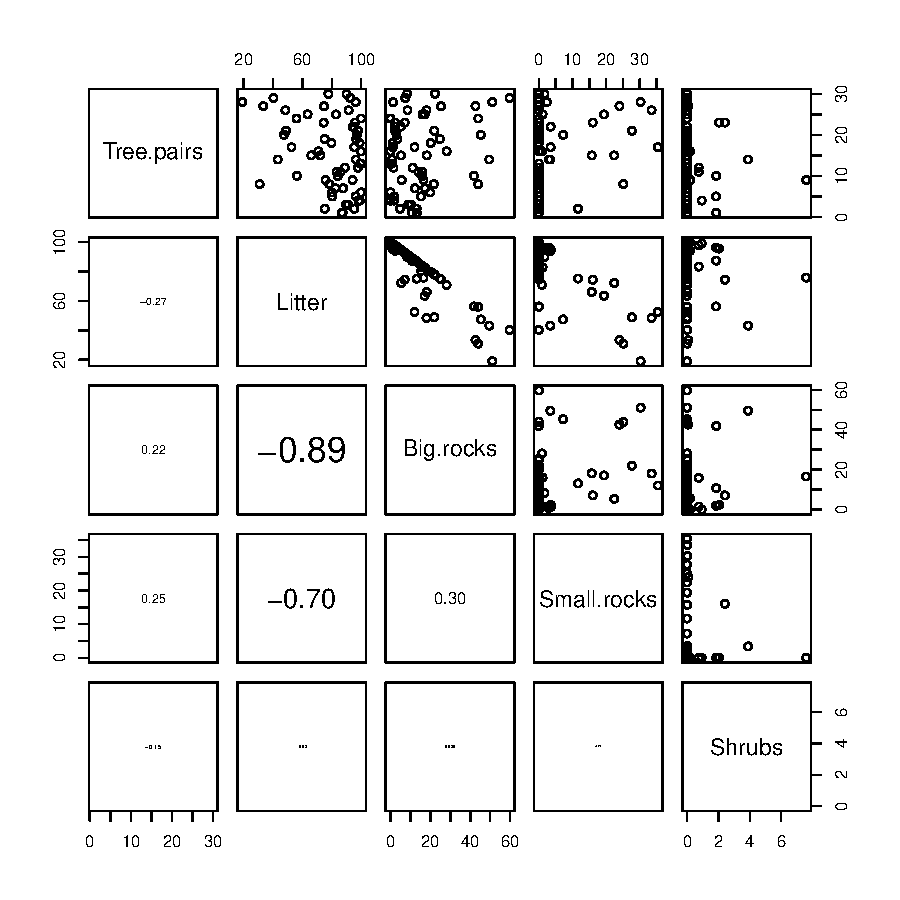
\includegraphics{SCRL-005}

\section{Community Response to Moth}

\subsection{Sampling}

\begin{Schunk}
\begin{Sinput}
> library(vegan)
> spac <- specaccum(com)
> plot(spac,xlab='Number of Trees',ylab='Number of Lichen Species')
> 
\end{Sinput}
\end{Schunk}

\subsection{Abundance, Richness and Diversity}

\begin{Schunk}
\begin{Sinput}
>                                         #abundance
> A <- apply(com,1,sum)
> A.fit <- glm(log(A+1)~Moth:Tree.pairs,data=env)
>                                         #richness
> R <- apply(com,1,function(x) length(x[x!=0]))
> R.fit <- glm(R~Moth:Tree.pairs,data=env,family='poisson')
>                                         #Shannon's diversity
> H <- apply(com,1,diversity)
> H.fit <- glm(H~Moth:Tree.pairs,data=env)
> 
\end{Sinput}
\end{Schunk}

\begin{Schunk}
\begin{Sinput}
> library(xtable)
> xtable(summary(A.fit))
\end{Sinput}
% latex table generated in R 2.15.0 by xtable 1.7-0 package
% Sat Jul  7 22:22:22 2012
\begin{table}[ht]
\begin{center}
\begin{tabular}{rrrrr}
  \hline
 & Estimate & Std. Error & t value & Pr($>$$|$t$|$) \\ 
  \hline
(Intercept) & 0.6388 & 0.1172 & 5.45 & 0.0000 \\ 
  Moth:Tree.pairs & 0.0182 & 0.0093 & 1.95 & 0.0555 \\ 
   \hline
\end{tabular}
\end{center}
\end{table}\begin{Sinput}
> xtable(summary(R.fit))
\end{Sinput}
% latex table generated in R 2.15.0 by xtable 1.7-0 package
% Sat Jul  7 22:22:22 2012
\begin{table}[ht]
\begin{center}
\begin{tabular}{rrrrr}
  \hline
 & Estimate & Std. Error & z value & Pr($>$$|$z$|$) \\ 
  \hline
(Intercept) & 1.3234 & 0.0832 & 15.91 & 0.0000 \\ 
  Moth:Tree.pairs & 0.0209 & 0.0057 & 3.66 & 0.0002 \\ 
   \hline
\end{tabular}
\end{center}
\end{table}\begin{Sinput}
> xtable(summary(H.fit))
\end{Sinput}
% latex table generated in R 2.15.0 by xtable 1.7-0 package
% Sat Jul  7 22:22:22 2012
\begin{table}[ht]
\begin{center}
\begin{tabular}{rrrrr}
  \hline
 & Estimate & Std. Error & t value & Pr($>$$|$t$|$) \\ 
  \hline
(Intercept) & 0.7461 & 0.1074 & 6.94 & 0.0000 \\ 
  Moth:Tree.pairs & 0.0205 & 0.0086 & 2.40 & 0.0197 \\ 
   \hline
\end{tabular}
\end{center}
\end{table}\begin{Sinput}
> 
\end{Sinput}
\end{Schunk}

\subsection{Composition}
\begin{Schunk}
\begin{Sinput}
>                                         #paired test of composition
> ds <- rep(min(com[com!=0]),nrow(com))
> com. <- cbind(com,ds)
> adonis(com.~env$Moth:env$Tree.pairs)
\end{Sinput}
\begin{Soutput}
Call:
adonis(formula = com. ~ env$Moth:env$Tree.pairs) 

Terms added sequentially (first to last)

                        Df SumsOfSqs MeanSqs F.Model      R2 Pr(>F)  
env$Moth:env$Tree.pairs  1    0.8211 0.82114  2.5772 0.04254  0.037 *
Residuals               58   18.4799 0.31862         0.95746         
Total                   59   19.3010                 1.00000         
---
Signif. codes:  0 ‘***’ 0.001 ‘**’ 0.01 ‘*’ 0.05 ‘.’ 0.1 ‘ ’ 1 
\end{Soutput}
\begin{Sinput}
> ##                                         #mvabund
> ## attach(env)
> ## mva.com <- com[,apply(com,2,sum)!=0]
> ##                                         #many glm with gaussian distribution
> ## mva.com <- apply(mva.com,2,sqrt)
> ## mva.com <- mvabund(mva.com)
> ## glm.fit <- manyglm(mva.com~Moth:Tree.pairs,family='gaussian')
> ## detach(env)
> ## anova(glm.fit)
> 
\end{Sinput}
\end{Schunk}

%% <<results=tex>>=
%% p.uni <- summary(glm.fit,p.uni='unadjusted')$uni.p
%% xtable(apply(p.uni,2,p.adjust,method='fdr'))

%% @ 

%% <<>>=
%% attach(env)
%% com.mglm <- manyglm(mva.com~Light.average*Litter*Big.rocks,family='gaussian')
%% detach(env)
%% summary(com.mglm)

%% @ 

\begin{Schunk}
\begin{Sinput}
>                                         #paired distance based
> d. <- as.matrix(vegdist(com.))
> pd <- 0
> for (i in 1:(nrow(d.)-1)){
+   pd[i] <- d.[(i+1),i]
+ }
> pd. <- pd[(1:length(pd)) %% 2 == 1]
> wilcox.test(pd.,exact=FALSE)
\end{Sinput}
\begin{Soutput}
	Wilcoxon signed rank test with continuity correction

data:  pd. 
V = 406, p-value = 4.003e-06
alternative hypothesis: true location is not equal to 0 
\end{Soutput}
\begin{Sinput}
> env.. <- env[(1:nrow(env)) %% 2 == 1,]
> library(tweedie)
> glm. <- glm(pd.~Light.average*Litter*Big.rocks,data=env..,family=tweedie(2))
> 
\end{Sinput}
\end{Schunk}

\begin{Schunk}
\begin{Sinput}
> xtable(summary(glm.))
\end{Sinput}
% latex table generated in R 2.15.0 by xtable 1.7-0 package
% Sat Jul  7 22:22:22 2012
\begin{table}[ht]
\begin{center}
\begin{tabular}{rrrrr}
  \hline
 & Estimate & Std. Error & t value & Pr($>$$|$t$|$) \\ 
  \hline
(Intercept) & -0.8025 & 3.4980 & -0.23 & 0.8207 \\ 
  Light.average & 0.1093 & 0.1556 & 0.70 & 0.4897 \\ 
  Litter & 0.0339 & 0.0395 & 0.86 & 0.4001 \\ 
  Big.rocks & 0.0378 & 0.0733 & 0.51 & 0.6117 \\ 
  Light.average:Litter & -0.0016 & 0.0017 & -0.91 & 0.3724 \\ 
  Light.average:Big.rocks & -0.0023 & 0.0031 & -0.76 & 0.4529 \\ 
  Litter:Big.rocks & -0.0007 & 0.0011 & -0.68 & 0.5009 \\ 
  Light.average:Litter:Big.rocks & 0.0000 & 0.0000 & 0.95 & 0.3503 \\ 
   \hline
\end{tabular}
\end{center}
\end{table}\begin{Sinput}
> 
\end{Sinput}
\end{Schunk}

\subsection{Indicator Species Analysis}

\begin{Schunk}
\begin{Sinput}
>                                         #indicator species
> ## library(labdsv)
> ## ind.spp <- indval(com,env$Moth)
> ## summary(ind.spp)
> ## detach(package:labdsv)
> 
\end{Sinput}
\end{Schunk}

\paragraph{} Indicator Species Analysis Results using Moth as the grouping factor
\paragraph{} species cluster indicator.value probability
\paragraph{} Canros       2          0.6397       0.006
\paragraph{} Acasup       2          0.6295       0.002
\paragraph{} Acacon       2          0.4769       0.001
\paragraph{} Acaobp       2          0.4241       0.008
\paragraph{} Phydub       2          0.4125       0.018
\paragraph{} Calare       2          0.2966       0.036


\begin{Schunk}
\begin{Sinput}
>                                         #NMDS
> library(ecodist)
> d <- vegdist(com.)
> if (any(ls()=='my.nmds')){}else{my.nmds <- nmds(d,3,3,100)}
\end{Sinput}
\begin{Soutput}
NULL
\end{Soutput}
\begin{Sinput}
> env.nms <- env.[,-c(3,4,5,6)]
> par(mfrow=c(3,3))
> for (i in 1:3){
+   for (j in 1:3){
+     if (i!=j){
+       par(mar=c(5.1, 4.1, 4.1, 2.1)-0.75)
+       vectors <- envfit(nmds.min(my.nmds)[,c(i,j)]~env.nms)
+       plot(nmds.min(my.nmds)[,c(j,i)],pch=19,col=grey(c(0.75,0))[(env$Moth+1)],xlab='',ylab='')
+       plot(vectors,col='black')
+     }else{
+       par(mar=c(5.1, 4.1, 4.1, 2.1)-2)
+       plot(1,1,axes=FALSE,xlab='',ylab='',type='n')
+       text(1,1,labels=paste('X',i,sep=''),cex=10)
+     }
+   }
+ }
\end{Sinput}
\begin{Soutput}
Minimum stress for given dimensionality:  0.1487555 
r^2 for minimum stress configuration:  0.8666012 
Minimum stress for given dimensionality:  0.1487555 
r^2 for minimum stress configuration:  0.8666012 
Minimum stress for given dimensionality:  0.1487555 
r^2 for minimum stress configuration:  0.8666012 
Minimum stress for given dimensionality:  0.1487555 
r^2 for minimum stress configuration:  0.8666012 
Minimum stress for given dimensionality:  0.1487555 
r^2 for minimum stress configuration:  0.8666012 
Minimum stress for given dimensionality:  0.1487555 
r^2 for minimum stress configuration:  0.8666012 
Minimum stress for given dimensionality:  0.1487555 
r^2 for minimum stress configuration:  0.8666012 
Minimum stress for given dimensionality:  0.1487555 
r^2 for minimum stress configuration:  0.8666012 
Minimum stress for given dimensionality:  0.1487555 
r^2 for minimum stress configuration:  0.8666012 
Minimum stress for given dimensionality:  0.1487555 
r^2 for minimum stress configuration:  0.8666012 
Minimum stress for given dimensionality:  0.1487555 
r^2 for minimum stress configuration:  0.8666012 
Minimum stress for given dimensionality:  0.1487555 
r^2 for minimum stress configuration:  0.8666012 
\end{Soutput}
\begin{Sinput}
> 
\end{Sinput}
\end{Schunk}
\includegraphics{SCRL-013}

%% <<>>=

%% attach(env)
%% com.mglm <- manyglm(mva.com~factor(Moth)*Light.average*Litter*Big.rocks,family='gaussian')
%% detach(env)
%% summary(com.mglm)

%% @ 

\pagebreak

\subsection{SEM}

%%SEM

\begin{Schunk}
\begin{Soutput}
 Model Chisquare =  5.0513   Df =  4 Pr(>Chisq) = 0.28207
 Chisquare (null model) =  158.65   Df =  10
 Goodness-of-fit index =  0.96765
 Adjusted goodness-of-fit index =  0.87868
 RMSEA index =  0.066744   90% CI: (NA, 0.21702)
 Bentler-Bonnett NFI =  0.96816
 Tucker-Lewis NNFI =  0.98232
 Bentler CFI =  0.99293
 SRMR =  0.039061
 AIC =  27.051
 AICc =  10.551
 BIC =  50.089
 CAIC =  -15.326

 Normalized Residuals
   Min. 1st Qu.  Median    Mean 3rd Qu.    Max. 
-0.9340  0.0000  0.0000 -0.0639  0.0297  0.3070 

 R-square for Endogenous Variables
Light.average        Litter     Abundance     Big.rocks 
       0.5583        0.1442        0.3360        0.7041 

 Parameter Estimates
      Estimate Std Error z value   Pr(>|z|)                                   
g.1.2  1.86246 0.215650    8.63652 5.7952e-18 Light.average <--- Moth         
g.1.3 -0.96225 0.305240   -3.15244 1.6191e-03 Litter <--- Moth                
b.2.5  0.26986 0.226461    1.19165 2.3340e-01 Abundance <--- Light.average    
b.3.4 -1.32422 0.111764  -11.84832 2.1954e-32 Big.rocks <--- Litter           
b.3.5  0.11105 0.397655    0.27926 7.8004e-01 Abundance <--- Litter           
b.4.5  0.74057 0.248775    2.97687 2.9121e-03 Abundance <--- Big.rocks        
e.1    0.25424 0.046809    5.43139 5.5917e-08 Moth <--> Moth                  
e.2    0.69757 0.128434    5.43139 5.5917e-08 Light.average <--> Light.average
e.3    1.39757 0.257314    5.43139 5.5917e-08 Litter <--> Litter              
e.4    1.20348 0.221579    5.43139 5.5917e-08 Big.rocks <--> Big.rocks        
e.5    4.39445 0.809084    5.43139 5.5917e-08 Abundance <--> Abundance        

 Iterations =  0 
\end{Soutput}
\begin{Soutput}
 5 largest modification indices, A matrix:
   Litter<-Light.average    Light.average<-Litter          Abundance<-Moth 
                2.494770                 2.494770                 1.254584 
    Big.rocks<-Abundance Big.rocks<-Light.average 
                1.137006                 1.137006 

  5 largest modification indices, P matrix:
   Light.average<->Litter          Abundance<->Moth Abundance<->Light.average 
                2.4947699                 1.2545837                 1.2545837 
       Abundance<->Litter          Big.rocks<->Moth 
                1.2545837                 0.8392215 
\end{Soutput}
\begin{Soutput}
Running  dot -Tpng -o semPathA.png  semPathA.dot 
\end{Soutput}
\end{Schunk}

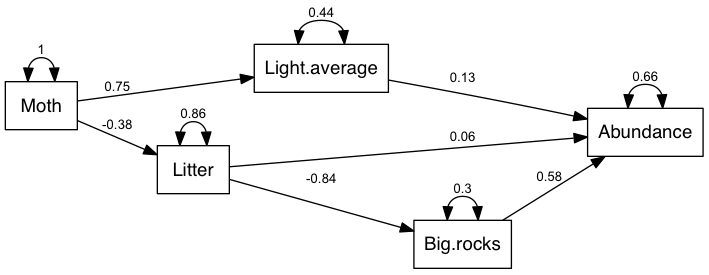
\includegraphics{semPathA.png}
\pagebreak

\begin{Schunk}
\begin{Soutput}
 Model Chisquare =  4.2927   Df =  4 Pr(>Chisq) = 0.36785
 Chisquare (null model) =  198.77   Df =  10
 Goodness-of-fit index =  0.9727
 Adjusted goodness-of-fit index =  0.89762
 RMSEA index =  0.035215   90% CI: (NA, 0.20261)
 Bentler-Bonnett NFI =  0.9784
 Tucker-Lewis NNFI =  0.99612
 Bentler CFI =  0.99845
 SRMR =  0.04022
 AIC =  26.293
 AICc =  9.7927
 BIC =  49.33
 CAIC =  -16.085

 Normalized Residuals
   Min. 1st Qu.  Median    Mean 3rd Qu.    Max. 
 -0.934  -0.216   0.000  -0.141   0.000   0.252 

 R-square for Endogenous Variables
Light.average        Litter      Richness     Big.rocks 
       0.5583        0.1442        0.6740        0.7041 

 Parameter Estimates
      Estimate Std Error z value  Pr(>|z|)                                   
g.1.2  1.86246 0.215650    8.6365 5.7952e-18 Light.average <--- Moth         
g.1.3 -0.96225 0.305240   -3.1524 1.6191e-03 Litter <--- Moth                
b.2.5  0.83401 0.200015    4.1697 3.0497e-05 Richness <--- Light.average     
b.3.4 -1.32422 0.111764  -11.8483 2.1954e-32 Big.rocks <--- Litter           
b.3.5  1.17773 0.351217    3.3533 7.9862e-04 Richness <--- Litter            
b.4.5  1.68066 0.219723    7.6490 2.0257e-14 Richness <--- Big.rocks         
e.1    0.25424 0.046809    5.4314 5.5917e-08 Moth <--> Moth                  
e.2    0.69757 0.128434    5.4314 5.5917e-08 Light.average <--> Light.average
e.3    1.39757 0.257314    5.4314 5.5917e-08 Litter <--> Litter              
e.4    1.20348 0.221579    5.4314 5.5917e-08 Big.rocks <--> Big.rocks        
e.5    3.42801 0.631147    5.4314 5.5917e-08 Richness <--> Richness          

 Iterations =  0 
\end{Soutput}
\begin{Soutput}
 5 largest modification indices, A matrix:
   Litter<-Light.average    Light.average<-Litter         Litter<-Richness 
                2.494770                 2.494770                 1.639637 
     Big.rocks<-Richness Big.rocks<-Light.average 
                1.137006                 1.137006 

  5 largest modification indices, P matrix:
  Light.average<->Litter         Big.rocks<->Moth       Big.rocks<->Litter 
               2.4947699                0.8392215                0.8392215 
         Richness<->Moth Richness<->Light.average 
               0.4628788                0.4628788 
\end{Soutput}
\begin{Soutput}
Running  dot -Tpng -o semPathR.png  semPathR.dot 
\end{Soutput}
\end{Schunk}

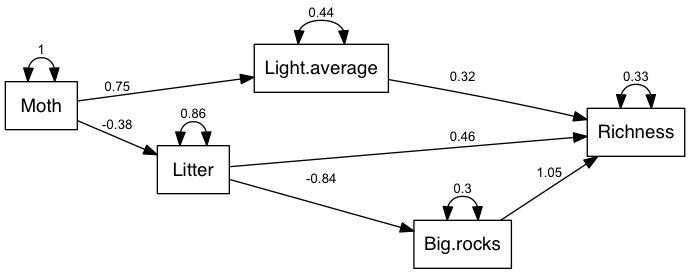
\includegraphics{semPathR.png}

\pagebreak

\begin{Schunk}
\begin{Soutput}
 Model Chisquare =  3.8579   Df =  4 Pr(>Chisq) = 0.42557
 Chisquare (null model) =  183.64   Df =  10
 Goodness-of-fit index =  0.97565
 Adjusted goodness-of-fit index =  0.90868
 RMSEA index =  0   90% CI: (NA, 0.19348)
 Bentler-Bonnett NFI =  0.97899
 Tucker-Lewis NNFI =  1.002
 Bentler CFI =  1
 SRMR =  0.042232
 AIC =  25.858
 AICc =  9.3579
 BIC =  48.896
 CAIC =  -16.519

 Normalized Residuals
   Min. 1st Qu.  Median    Mean 3rd Qu.    Max. 
 -0.934  -0.271   0.000  -0.156   0.000   0.252 

 R-square for Endogenous Variables
Light.average        Litter     Diversity     Big.rocks 
       0.5583        0.1442        0.5808        0.7041 

 Parameter Estimates
      Estimate Std Error z value  Pr(>|z|)                                   
g.1.2  1.86246 0.215650    8.6365 5.7952e-18 Light.average <--- Moth         
g.1.3 -0.96225 0.305240   -3.1524 1.6191e-03 Litter <--- Moth                
b.2.5  0.16786 0.047902    3.5042 4.5794e-04 Diversity <--- Light.average    
b.3.4 -1.32422 0.111764  -11.8483 2.1954e-32 Big.rocks <--- Litter           
b.3.5  0.22462 0.084115    2.6704 7.5763e-03 Diversity <--- Litter           
b.4.5  0.32511 0.052622    6.1782 6.4842e-10 Diversity <--- Big.rocks        
e.1    0.25424 0.046809    5.4314 5.5917e-08 Moth <--> Moth                  
e.2    0.69757 0.128434    5.4314 5.5917e-08 Light.average <--> Light.average
e.3    1.39757 0.257314    5.4314 5.5917e-08 Litter <--> Litter              
e.4    1.20348 0.221579    5.4314 5.5917e-08 Big.rocks <--> Big.rocks        
e.5    0.19662 0.036201    5.4314 5.5917e-08 Diversity <--> Diversity        

 Iterations =  0 
\end{Soutput}
\begin{Soutput}
 5 largest modification indices, A matrix:
   Light.average<-Litter    Litter<-Light.average        Litter<-Diversity 
                2.494770                 2.494770                 2.420293 
Big.rocks<-Light.average     Big.rocks<-Diversity 
                1.137006                 1.137006 

  5 largest modification indices, P matrix:
   Light.average<->Litter          Big.rocks<->Moth        Big.rocks<->Litter 
               2.49476987                0.83922155                0.83922155 
Light.average<->Big.rocks        Diversity<->Litter 
               0.34301774                0.00461226 
\end{Soutput}
\begin{Soutput}
Running  dot -Tpng -o semPathD.png  semPathD.dot 
\end{Soutput}
\end{Schunk}

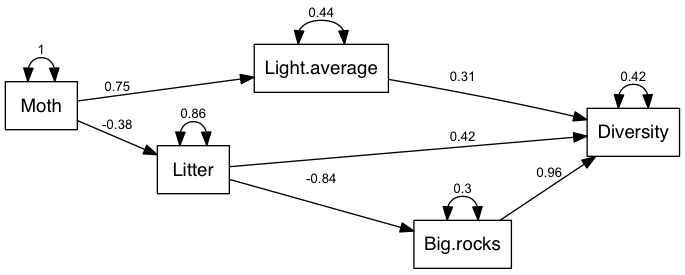
\includegraphics{semPathD.png}

\pagebreak

\begin{Schunk}
\begin{Soutput}
Minimum stress for given dimensionality:  0.1487555 
r^2 for minimum stress configuration:  0.8666012 
\end{Soutput}
\begin{Soutput}
 Model Chisquare =  8.4011   Df =  9 Pr(>Chisq) = 0.49428
 Chisquare (null model) =  203.09   Df =  21
 Goodness-of-fit index =  0.95968
 Adjusted goodness-of-fit index =  0.87455
 RMSEA index =  0   90% CI: (NA, 0.13967)
 Bentler-Bonnett NFI =  0.95863
 Tucker-Lewis NNFI =  1.0077
 Bentler CFI =  1
 SRMR =  0.047869
 AIC =  46.401
 AICc =  27.401
 BIC =  86.194
 CAIC =  -37.448

 Normalized Residuals
   Min. 1st Qu.  Median    Mean 3rd Qu.    Max. 
-0.9340 -0.1790  0.0000 -0.0171  0.1080  0.8890 

 R-square for Endogenous Variables
Light.average        Litter            X1            X2            X3 
       0.5583        0.1442        0.4217        0.4097        0.0521 
    Big.rocks 
       0.7041 

 Parameter Estimates
      Estimate  Std Error z value   Pr(>|z|)                                   
g.1.2  1.862463 0.215650    8.63652 5.7952e-18 Light.average <--- Moth         
g.1.3 -0.962252 0.305240   -3.15244 1.6191e-03 Litter <--- Moth                
b.2.5 -0.080703 0.029471   -2.73840 6.1739e-03 X1 <--- Light.average           
b.2.6  0.054260 0.027169    1.99716 4.5808e-02 X2 <--- Light.average           
b.2.7 -0.026432 0.031000   -0.85264 3.9386e-01 X3 <--- Light.average           
b.3.4 -1.324220 0.111764  -11.84832 2.1954e-32 Big.rocks <--- Litter           
b.3.5 -0.160718 0.051750   -3.10569 1.8984e-03 X1 <--- Litter                  
b.3.6  0.067605 0.047707    1.41709 1.5646e-01 X2 <--- Litter                  
b.3.7  0.074578 0.054434    1.37007 1.7067e-01 X3 <--- Litter                  
b.4.5 -0.167030 0.032375   -5.15927 2.4791e-07 X1 <--- Big.rocks               
b.4.6  0.124920 0.029846    4.18552 2.8451e-05 X2 <--- Big.rocks               
b.4.7  0.035507 0.034054    1.04266 2.9711e-01 X3 <--- Big.rocks               
e.1    0.254237 0.046809    5.43139 5.5917e-08 Moth <--> Moth                  
e.2    0.697573 0.128434    5.43139 5.5917e-08 Light.average <--> Light.average
e.3    1.397574 0.257314    5.43139 5.5917e-08 Litter <--> Litter              
e.4    1.203481 0.221579    5.43139 5.5917e-08 Big.rocks <--> Big.rocks        
e.5    0.074423 0.013702    5.43139 5.5917e-08 X1 <--> X1                      
e.6    0.063249 0.011645    5.43139 5.5917e-08 X2 <--> X2                      
e.7    0.082344 0.015161    5.43139 5.5917e-08 X3 <--> X3                      

 Iterations =  0 
\end{Soutput}
\begin{Soutput}
 5 largest modification indices, A matrix:
           Litter<-X1 Litter<-Light.average Light.average<-Litter 
             3.438300              2.494770              2.494770 
               X1<-X2                X2<-X1 
             2.245427              2.245427 

  5 largest modification indices, P matrix:
Light.average<->Litter                X2<->X1              X2<->Moth 
              2.494770               2.245427               1.144694 
    X2<->Light.average            X2<->Litter 
              1.144694               1.144694 
\end{Soutput}
\begin{Soutput}
Running  dot -Tpng -o semPath1.png  semPath1.dot 
\end{Soutput}
\end{Schunk}

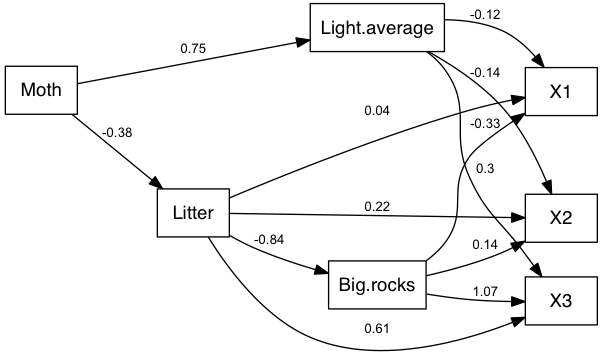
\includegraphics{semPath1.png}

\begin{Schunk}
\begin{Soutput}
 Model Chisquare =  3.9132   Df =  4 Pr(>Chisq) = 0.41787
 Chisquare (null model) =  166.87   Df =  10
 Goodness-of-fit index =  0.97527
 Adjusted goodness-of-fit index =  0.90726
 RMSEA index =  0   90% CI: (NA, 0.19468)
 Bentler-Bonnett NFI =  0.97655
 Tucker-Lewis NNFI =  1.0014
 Bentler CFI =  1
 SRMR =  0.04181
 AIC =  25.913
 AICc =  9.4132
 BIC =  48.951
 CAIC =  -16.464

 Normalized Residuals
   Min. 1st Qu.  Median    Mean 3rd Qu.    Max. 
-0.9340  0.0000  0.0000 -0.0575  0.0736  0.4100 

 R-square for Endogenous Variables
Light.average        Litter        Acacon     Big.rocks 
       0.5583        0.1442        0.4175        0.7041 

 Parameter Estimates
      Estimate   Std Error z value   Pr(>|z|)  
g.1.2  1.8624634 0.2156498   8.63652 5.7952e-18
g.1.3 -0.9622521 0.3052403  -3.15244 1.6191e-03
b.2.5  0.0119617 0.0045513   2.62819 8.5840e-03
b.3.4 -1.3242197 0.1117643 -11.84832 2.1954e-32
b.3.5 -0.0186545 0.0079919  -2.33419 1.9586e-02
b.4.5  0.0025973 0.0049998   0.51949 6.0342e-01
e.1    0.2542373 0.0468089   5.43139 5.5917e-08
e.2    0.6975726 0.1284335   5.43139 5.5917e-08
e.3    1.3975744 0.2573143   5.43139 5.5917e-08
e.4    1.2034807 0.2215787   5.43139 5.5917e-08
e.5    0.0017750 0.0003268   5.43139 5.5917e-08
                                      
g.1.2 Light.average <--- Moth         
g.1.3 Litter <--- Moth                
b.2.5 Acacon <--- Light.average       
b.3.4 Big.rocks <--- Litter           
b.3.5 Acacon <--- Litter              
b.4.5 Acacon <--- Big.rocks           
e.1   Moth <--> Moth                  
e.2   Light.average <--> Light.average
e.3   Litter <--> Litter              
e.4   Big.rocks <--> Big.rocks        
e.5   Acacon <--> Acacon              

 Iterations =  0 
\end{Soutput}
\begin{Soutput}
 5 largest modification indices, A matrix:
   Litter<-Light.average    Light.average<-Litter Big.rocks<-Light.average 
               2.4947699                2.4947699                1.1370060 
       Big.rocks<-Acacon Light.average<-Big.rocks 
               1.1370060                0.9165941 

  5 largest modification indices, P matrix:
   Light.average<->Litter        Big.rocks<->Litter          Big.rocks<->Moth 
               2.49476987                0.83922155                0.83922155 
Light.average<->Big.rocks           Acacon<->Litter 
               0.34301774                0.06310573 
\end{Soutput}
\begin{Soutput}
Running  dot -Tpng -o semPathAcacon.png  semPathAcacon.dot 
\end{Soutput}
\end{Schunk}

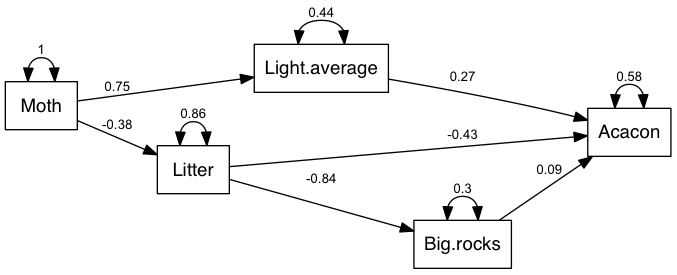
\includegraphics{semPathAcacon.png}

\pagebreak

\begin{Schunk}
\begin{Soutput}
 Model Chisquare =  3.9045   Df =  4 Pr(>Chisq) = 0.41908
 Chisquare (null model) =  185.53   Df =  10
 Goodness-of-fit index =  0.97533
 Adjusted goodness-of-fit index =  0.90749
 RMSEA index =  0   90% CI: (NA, 0.19449)
 Bentler-Bonnett NFI =  0.97896
 Tucker-Lewis NNFI =  1.0014
 Bentler CFI =  1
 SRMR =  0.04161
 AIC =  25.905
 AICc =  9.4045
 BIC =  48.942
 CAIC =  -16.473

 Normalized Residuals
   Min. 1st Qu.  Median    Mean 3rd Qu.    Max. 
-0.9340 -0.1620  0.0000 -0.0840  0.0431  0.3860 

 R-square for Endogenous Variables
Light.average        Litter        Acasup     Big.rocks 
       0.5583        0.1442        0.5794        0.7041 

 Parameter Estimates
      Estimate  Std Error z value  Pr(>|z|)                                   
g.1.2  1.862463 0.2156498   8.6365 5.7952e-18 Light.average <--- Moth         
g.1.3 -0.962252 0.3052403  -3.1524 1.6191e-03 Litter <--- Moth                
b.2.5  0.036276 0.0156584   2.3167 2.0521e-02 Acasup <--- Light.average       
b.3.4 -1.324220 0.1117643 -11.8483 2.1954e-32 Big.rocks <--- Litter           
b.3.5 -0.056637 0.0274954  -2.0599 3.9411e-02 Acasup <--- Litter              
b.4.5  0.042716 0.0172013   2.4833 1.3017e-02 Acasup <--- Big.rocks           
e.1    0.254237 0.0468089   5.4314 5.5917e-08 Moth <--> Moth                  
e.2    0.697573 0.1284335   5.4314 5.5917e-08 Light.average <--> Light.average
e.3    1.397574 0.2573143   5.4314 5.5917e-08 Litter <--> Litter              
e.4    1.203481 0.2215787   5.4314 5.5917e-08 Big.rocks <--> Big.rocks        
e.5    0.021009 0.0038681   5.4314 5.5917e-08 Acasup <--> Acasup              

 Iterations =  0 
\end{Soutput}
\begin{Soutput}
 5 largest modification indices, A matrix:
   Light.average<-Litter    Litter<-Light.average           Litter<-Acasup 
                2.494770                 2.494770                 1.982069 
   Light.average<-Acasup Big.rocks<-Light.average 
                1.397081                 1.137006 

  5 largest modification indices, P matrix:
   Light.average<->Litter          Big.rocks<->Moth        Big.rocks<->Litter 
               2.49476987                0.83922155                0.83922155 
Light.average<->Big.rocks           Acasup<->Litter 
               0.34301774                0.05389307 
\end{Soutput}
\begin{Soutput}
Running  dot -Tpng -o semPathAcasup.png  semPathAcasup.dot 
\end{Soutput}
\end{Schunk}

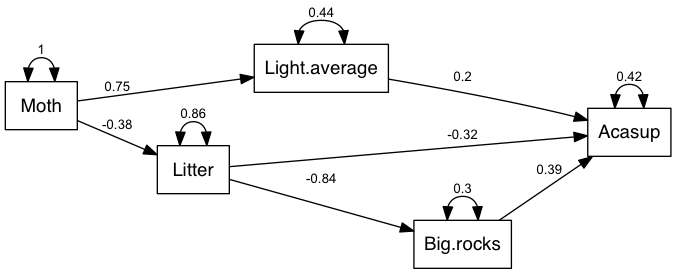
\includegraphics{semPathAcasup.png}

\pagebreak

\begin{Schunk}
\begin{Soutput}
 Model Chisquare =  3.8536   Df =  3 Pr(>Chisq) = 0.27772
 Chisquare (null model) =  142.14   Df =  10
 Goodness-of-fit index =  0.97568
 Adjusted goodness-of-fit index =  0.87839
 RMSEA index =  0.069444   90% CI: (NA, 0.24056)
 Bentler-Bonnett NFI =  0.97289
 Tucker-Lewis NNFI =  0.97847
 Bentler CFI =  0.99354
 SRMR =  0.042811
 AIC =  27.854
 AICc =  10.492
 BIC =  52.986
 CAIC =  -11.429

 Normalized Residuals
   Min. 1st Qu.  Median    Mean 3rd Qu.    Max. 
-0.9340 -0.0505  0.0000 -0.0853  0.0000  0.5020 

 R-square for Endogenous Variables
Light.average        Litter        Acaobp     Big.rocks 
       0.5583        0.1442        0.1465        0.7041 

 Parameter Estimates
      Estimate  Std Error z value   Pr(>|z|)                                   
g.1.2  1.862463 0.215650    8.63652 5.7952e-18 Light.average <--- Moth         
g.1.3 -0.962252 0.305240   -3.15244 1.6191e-03 Litter <--- Moth                
g.1.5  1.056837 0.384638    2.74761 6.0030e-03 Acaobp <--- Moth                
b.2.5 -0.427636 0.148880   -2.87236 4.0742e-03 Acaobp <--- Light.average       
b.3.4 -1.324220 0.111764  -11.84832 2.1954e-32 Big.rocks <--- Litter           
b.3.5  0.034415 0.183282    0.18777 8.5106e-01 Acaobp <--- Litter              
b.4.5  0.056794 0.113347    0.50106 6.1633e-01 Acaobp <--- Big.rocks           
e.1    0.254237 0.046809    5.43139 5.5917e-08 Moth <--> Moth                  
e.2    0.697573 0.128434    5.43139 5.5917e-08 Light.average <--> Light.average
e.3    1.397574 0.257314    5.43139 5.5917e-08 Litter <--> Litter              
e.4    1.203481 0.221579    5.43139 5.5917e-08 Big.rocks <--> Big.rocks        
e.5    0.912248 0.167958    5.43139 5.5917e-08 Acaobp <--> Acaobp              

 Iterations =  0 
\end{Soutput}
\begin{Soutput}
 5 largest modification indices, A matrix:
   Light.average<-Litter    Litter<-Light.average           Litter<-Acaobp 
               2.4947699                2.4947699                2.2967054 
Big.rocks<-Light.average Light.average<-Big.rocks 
               1.1370060                0.9165941 

  5 largest modification indices, P matrix:
   Light.average<->Litter          Big.rocks<->Moth        Big.rocks<->Litter 
                2.4947699                 0.8392215                 0.8392215 
Light.average<->Big.rocks                      <NA> 
                0.3430177                        NA 
\end{Soutput}
\begin{Soutput}
Running  dot -Tpng -o semPathAcaobp.png  semPathAcaobp.dot 
\end{Soutput}
\end{Schunk}

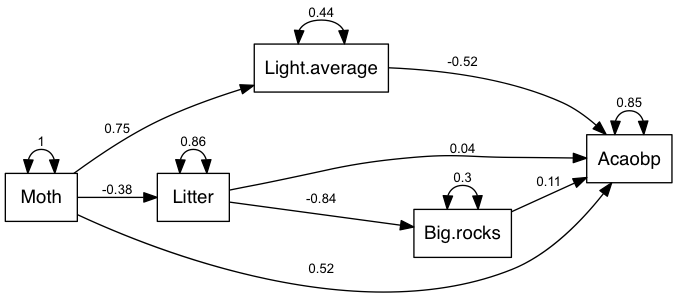
\includegraphics{semPathAcaobp.png}
\pagebreak

\begin{Schunk}
\begin{Soutput}
 Model Chisquare =  3.8661   Df =  4 Pr(>Chisq) = 0.42443
 Chisquare (null model) =  191.38   Df =  10
 Goodness-of-fit index =  0.97559
 Adjusted goodness-of-fit index =  0.90847
 RMSEA index =  0   90% CI: (NA, 0.19366)
 Bentler-Bonnett NFI =  0.9798
 Tucker-Lewis NNFI =  1.0018
 Bentler CFI =  1
 SRMR =  0.040632
 AIC =  25.866
 AICc =  9.3661
 BIC =  48.904
 CAIC =  -16.511

 Normalized Residuals
   Min. 1st Qu.  Median    Mean 3rd Qu.    Max. 
-0.9340 -0.2020  0.0000 -0.1080  0.0802  0.2520 

 R-square for Endogenous Variables
Light.average        Litter        Canros     Big.rocks 
       0.5583        0.1442        0.6211        0.7041 

 Parameter Estimates
      Estimate   Std Error z value   Pr(>|z|)  
g.1.2  1.8624634 0.215650    8.63652 5.7952e-18
g.1.3 -0.9622521 0.305240   -3.15244 1.6191e-03
b.2.5  0.1295623 0.028641    4.52371 6.0765e-06
b.3.4 -1.3242197 0.111764  -11.84832 2.1954e-32
b.3.5 -0.0083869 0.050292   -0.16676 8.6756e-01
b.4.5  0.1249703 0.031463    3.97200 7.1271e-05
e.1    0.2542373 0.046809    5.43139 5.5917e-08
e.2    0.6975726 0.128434    5.43139 5.5917e-08
e.3    1.3975744 0.257314    5.43139 5.5917e-08
e.4    1.2034807 0.221579    5.43139 5.5917e-08
e.5    0.0702887 0.012941    5.43139 5.5917e-08
                                      
g.1.2 Light.average <--- Moth         
g.1.3 Litter <--- Moth                
b.2.5 Canros <--- Light.average       
b.3.4 Big.rocks <--- Litter           
b.3.5 Canros <--- Litter              
b.4.5 Canros <--- Big.rocks           
e.1   Moth <--> Moth                  
e.2   Light.average <--> Light.average
e.3   Litter <--> Litter              
e.4   Big.rocks <--> Big.rocks        
e.5   Canros <--> Canros              

 Iterations =  0 
\end{Soutput}
\begin{Soutput}
 5 largest modification indices, A matrix:
   Light.average<-Litter    Litter<-Light.average           Litter<-Canros 
                2.494770                 2.494770                 2.299203 
Big.rocks<-Light.average        Big.rocks<-Canros 
                1.137006                 1.137006 

  5 largest modification indices, P matrix:
   Light.average<->Litter          Big.rocks<->Moth        Big.rocks<->Litter 
               2.49476987                0.83922155                0.83922155 
Light.average<->Big.rocks             Canros<->Moth 
               0.34301774                0.01323831 
\end{Soutput}
\begin{Soutput}
Running  dot -Tpng -o semPathCanros.png  semPathCanros.dot 
\end{Soutput}
\end{Schunk}


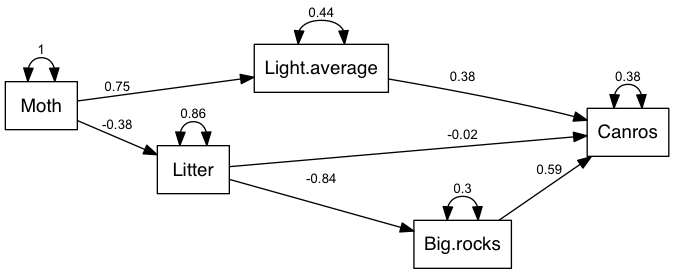
\includegraphics{semPathCanros.png}
\pagebreak

\begin{Schunk}
\begin{Soutput}
 Model Chisquare =  5.0461   Df =  4 Pr(>Chisq) = 0.2826
 Chisquare (null model) =  138.66   Df =  10
 Goodness-of-fit index =  0.96768
 Adjusted goodness-of-fit index =  0.87881
 RMSEA index =  0.066579   90% CI: (NA, 0.21693)
 Bentler-Bonnett NFI =  0.96361
 Tucker-Lewis NNFI =  0.97967
 Bentler CFI =  0.99187
 SRMR =  0.042323
 AIC =  27.046
 AICc =  10.546
 BIC =  50.084
 CAIC =  -15.331

 Normalized Residuals
   Min. 1st Qu.  Median    Mean 3rd Qu.    Max. 
-0.9340 -0.1910  0.0000 -0.0819  0.0000  0.5010 

 R-square for Endogenous Variables
Light.average        Litter        Calare     Big.rocks 
       0.5583        0.1442        0.0825        0.7041 

 Parameter Estimates
      Estimate   Std Error  z value  Pr(>|z|)  
g.1.2  1.8624634 0.21564981   8.6365 5.7952e-18
g.1.3 -0.9622521 0.30524028  -3.1524 1.6191e-03
b.2.5  0.0117248 0.00774787   1.5133 1.3021e-01
b.3.4 -1.3242197 0.11176430 -11.8483 2.1954e-32
b.3.5  0.0202336 0.01360492   1.4872 1.3696e-01
b.4.5  0.0145328 0.00851130   1.7075 8.7735e-02
e.1    0.2542373 0.04680888   5.4314 5.5917e-08
e.2    0.6975726 0.12843352   5.4314 5.5917e-08
e.3    1.3975744 0.25731430   5.4314 5.5917e-08
e.4    1.2034807 0.22157875   5.4314 5.5917e-08
e.5    0.0051438 0.00094705   5.4314 5.5917e-08
                                      
g.1.2 Light.average <--- Moth         
g.1.3 Litter <--- Moth                
b.2.5 Calare <--- Light.average       
b.3.4 Big.rocks <--- Litter           
b.3.5 Calare <--- Litter              
b.4.5 Calare <--- Big.rocks           
e.1   Moth <--> Moth                  
e.2   Light.average <--> Light.average
e.3   Litter <--> Litter              
e.4   Big.rocks <--> Big.rocks        
e.5   Calare <--> Calare              

 Iterations =  0 
\end{Soutput}
\begin{Soutput}
 5 largest modification indices, A matrix:
Light.average<-Litter Litter<-Light.average Light.average<-Calare 
             2.494770              2.494770              1.624254 
         Calare<-Moth     Big.rocks<-Calare 
             1.249195              1.137006 

  5 largest modification indices, P matrix:
Light.average<->Litter        Calare<->Litter Calare<->Light.average 
             2.4947699              1.2491953              1.2491953 
         Calare<->Moth       Big.rocks<->Moth 
             1.2491953              0.8392215 
\end{Soutput}
\begin{Soutput}
Running  dot -Tpng -o semPathCalare.png  semPathCalare.dot 
\end{Soutput}
\end{Schunk}


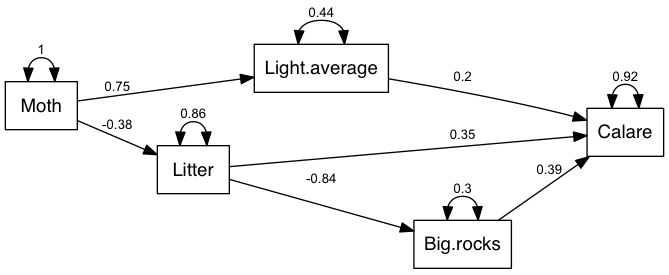
\includegraphics{semPathCalare.png}
\pagebreak

\begin{Schunk}
\begin{Soutput}
 Model Chisquare =  4.5   Df =  4 Pr(>Chisq) = 0.34255
 Chisquare (null model) =  146.05   Df =  10
 Goodness-of-fit index =  0.97131
 Adjusted goodness-of-fit index =  0.8924
 RMSEA index =  0.046028   90% CI: (NA, 0.20672)
 Bentler-Bonnett NFI =  0.96919
 Tucker-Lewis NNFI =  0.99081
 Bentler CFI =  0.99633
 SRMR =  0.039249
 AIC =  26.5
 AICc =  10
 BIC =  49.538
 CAIC =  -15.877

 Normalized Residuals
   Min. 1st Qu.  Median    Mean 3rd Qu.    Max. 
 -0.934  -0.189   0.000  -0.105   0.000   0.252 

 R-square for Endogenous Variables
Light.average        Litter        Phydub     Big.rocks 
       0.5583        0.1442        0.1979        0.7041 

 Parameter Estimates
      Estimate  Std Error z value  Pr(>|z|)                                   
g.1.2  1.862463 0.2156498   8.6365 5.7952e-18 Light.average <--- Moth         
g.1.3 -0.962252 0.3052403  -3.1524 1.6191e-03 Litter <--- Moth                
b.2.5  0.038712 0.0204195   1.8959 5.7979e-02 Phydub <--- Light.average       
b.3.4 -1.324220 0.1117643 -11.8483 2.1954e-32 Big.rocks <--- Litter           
b.3.5  0.059666 0.0358558   1.6640 9.6103e-02 Phydub <--- Litter              
b.4.5  0.062696 0.0224315   2.7950 5.1903e-03 Phydub <--- Big.rocks           
e.1    0.254237 0.0468089   5.4314 5.5917e-08 Moth <--> Moth                  
e.2    0.697573 0.1284335   5.4314 5.5917e-08 Light.average <--> Light.average
e.3    1.397574 0.2573143   5.4314 5.5917e-08 Litter <--> Litter              
e.4    1.203481 0.2215787   5.4314 5.5917e-08 Big.rocks <--> Big.rocks        
e.5    0.035728 0.0065781   5.4314 5.5917e-08 Phydub <--> Phydub              

 Iterations =  0 
\end{Soutput}
\begin{Soutput}
 5 largest modification indices, A matrix:
   Litter<-Light.average    Light.average<-Litter        Big.rocks<-Phydub 
               2.4947699                2.4947699                1.1370060 
Big.rocks<-Light.average Light.average<-Big.rocks 
               1.1370060                0.9165941 

  5 largest modification indices, P matrix:
Light.average<->Litter       Big.rocks<->Moth     Big.rocks<->Litter 
             2.4947699              0.8392215              0.8392215 
Phydub<->Light.average          Phydub<->Moth 
             0.6802393              0.6802393 
\end{Soutput}
\begin{Soutput}
Running  dot -Tpng -o semPathPhydub.png  semPathPhydub.dot 
\end{Soutput}
\end{Schunk}

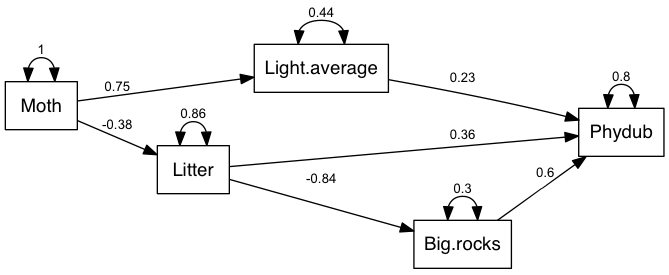
\includegraphics{semPathPhydub.png}
\pagebreak

\begin{Schunk}
\begin{Sinput}
>                                         #co-occurrence null models
> library(bipartite)
> source('~/cor_nets/CorNets.R')
> library(audio)
>                                         #all
> x <- com
> if (any(ls()=='null')){}else{null <- nullSim(x,10000)}
\end{Sinput}
\begin{Soutput}
NULL
\end{Soutput}
\begin{Sinput}
> length(null)
\end{Sinput}
\begin{Soutput}
[1] 10000
\end{Soutput}
\begin{Sinput}
> if (any(ls()=='null.all')){}else{sim <- lapply(null,C.score);null.all <- unlist(sim)}
\end{Sinput}
\begin{Soutput}
NULL
\end{Soutput}
\begin{Sinput}
> p.all <- min(c(length(sim[sim>=C.score(x)])/length(sim),length(sim[sim<=C.score(x)])/length(sim)))
> ses.all <- (C.score(x) - mean(sim)) / sd(sim)
>                                         #moth susceptible
> x <- com[env$Moth==0,]
> if (any(ls()=='null')){}else{null <- nullSim(x,10000)}
\end{Sinput}
\begin{Soutput}
NULL
\end{Soutput}
\begin{Sinput}
> length(null)
\end{Sinput}
\begin{Soutput}
[1] 10000
\end{Soutput}
\begin{Sinput}
> if (any(ls()=='null.0')){}else{sim <- lapply(null,C.score);null.0 <- unlist(sim)}
\end{Sinput}
\begin{Soutput}
NULL
\end{Soutput}
\begin{Sinput}
> p.0 <- min(c(length(sim[sim>=C.score(x)])/length(sim),length(sim[sim<=C.score(x)])/length(sim)))
> ses.0 <- (C.score(x) - mean(sim)) / sd(sim)
>                                         #moth resistant
> x <- com[env$Moth==1,]
> if (any(ls()=='null')){}else{null <- nullSim(x,10000)}
\end{Sinput}
\begin{Soutput}
NULL
\end{Soutput}
\begin{Sinput}
> length(null)
\end{Sinput}
\begin{Soutput}
[1] 10000
\end{Soutput}
\begin{Sinput}
> if (any(ls()=='null.1')){}else{sim <- lapply(null,C.score);null.1 <- unlist(sim)}
\end{Sinput}
\begin{Soutput}
NULL
\end{Soutput}
\begin{Sinput}
> p.1 <- min(c(length(sim[sim>=C.score(x)])/length(sim),length(sim[sim<=C.score(x)])/length(sim)))
> ses.1 <- (C.score(x) - mean(sim)) / sd(sim)
>                                         #compare co-occurrence patterns
> cooc <- cbind(c(p.0,ses.0),c(p.1,ses.1),c(p.all,ses.all))
> colnames(cooc) <- c('S','R','ALL')
> rownames(cooc) <- c('p.min','SES')
> cooc
\end{Sinput}
\begin{Soutput}
             S         R        ALL
p.min 0.171600  0.049900  0.2852000
SES   0.892948 -1.574635 -0.5934756
\end{Soutput}
\begin{Sinput}
> 
\end{Sinput}
\end{Schunk}

\begin{Schunk}
\begin{Sinput}
> library(xtable)
> xtable(cooc)
\end{Sinput}
% latex table generated in R 2.15.0 by xtable 1.7-0 package
% Sat Jul  7 22:22:25 2012
\begin{table}[ht]
\begin{center}
\begin{tabular}{rrrr}
  \hline
 & S & R & ALL \\ 
  \hline
p.min & 0.17 & 0.05 & 0.29 \\ 
  SES & 0.89 & -1.57 & -0.59 \\ 
   \hline
\end{tabular}
\end{center}
\end{table}\begin{Sinput}
> 
\end{Sinput}
\end{Schunk}

\begin{Schunk}
\begin{Sinput}
>                                         #co-occurrence network
> source('~/cor_nets/araujo_method/araujo_method.R')
> library(sna)
> x.net <- cbind(env$Moth,com)
> names(x.net)[1] <- 'moth'
> if (any(ls()=='net')){}else{net <- araujoNet(x.net)$dp}
\end{Sinput}
\begin{Soutput}
NULL
\end{Soutput}
\begin{Sinput}
> if (any(ls()=='net.0')){}else{net.0 <- araujoNet(x.net[env$Moth==0,])$dp}
\end{Sinput}
\begin{Soutput}
NULL
\end{Soutput}
\begin{Sinput}
> if (any(ls()=='net.1')){}else{net.1 <- araujoNet(x.net[env$Moth==1,])$dp}
\end{Sinput}
\begin{Soutput}
NULL
\end{Soutput}
\begin{Sinput}
> par(mfrow=c(2,3))
> gplot(net,gmode='graph',displaylabels=TRUE,label.cex=0.65)
> gplot(net.0,gmode='graph',displaylabels=TRUE,label.cex=0.65)
> gplot(net.1,gmode='graph',displaylabels=TRUE,label.cex=0.65)
> hist(null.all)
> abline(v=C.score(com))
> hist(null.0)
> abline(v=C.score(com[env$Moth==0,]))
> hist(null.1)
> abline(v=C.score(com[env$Moth==1,]))
> 
\end{Sinput}
\end{Schunk}
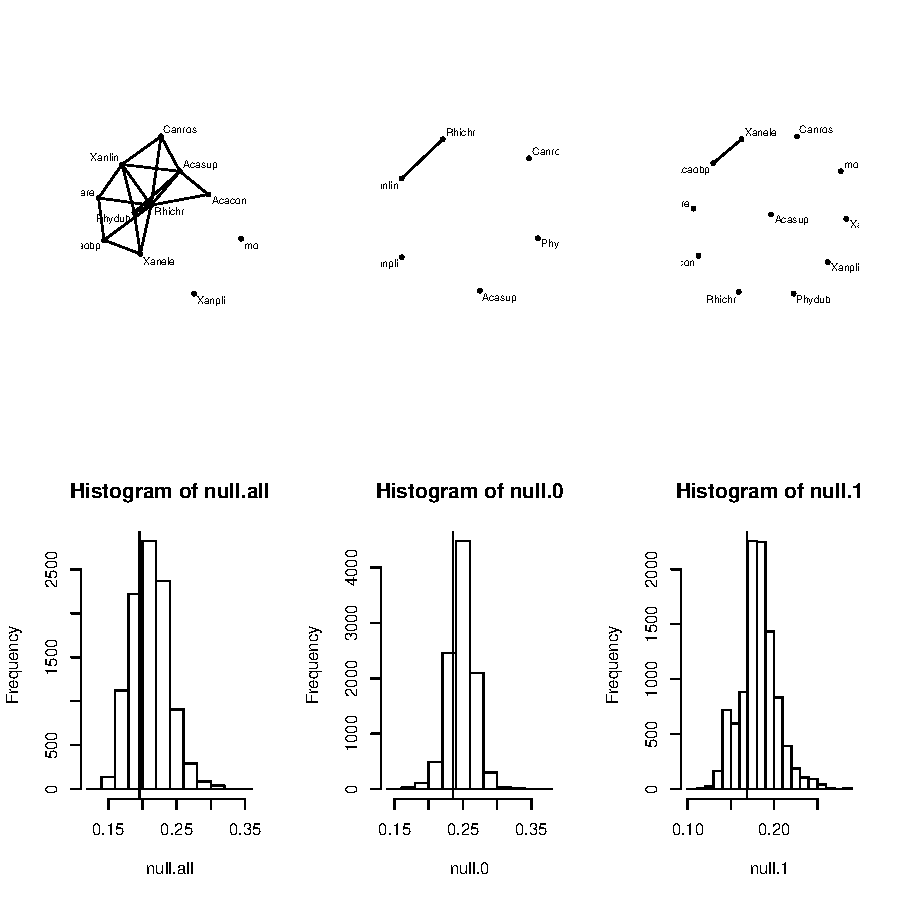
\includegraphics{SCRL-026}

\begin{Schunk}
\begin{Sinput}
> e.col <- net
> e.col[net!=0] <- 'grey'
> v.cex <- apply(x.net,2,function(x) length(x[x!=0]))
> v.cex <- (v.cex / max(v.cex) + 1)^2
> gplot(net,gmode='graph',displaylabels=TRUE,label.cex=0.65,
+       edge.col=e.col,edge.lwd=(net+1)^10,vertex.cex=v.cex,
+       vertex.sides=50,vertex.col='black',vertex.border='white')
> 
\end{Sinput}
\end{Schunk}
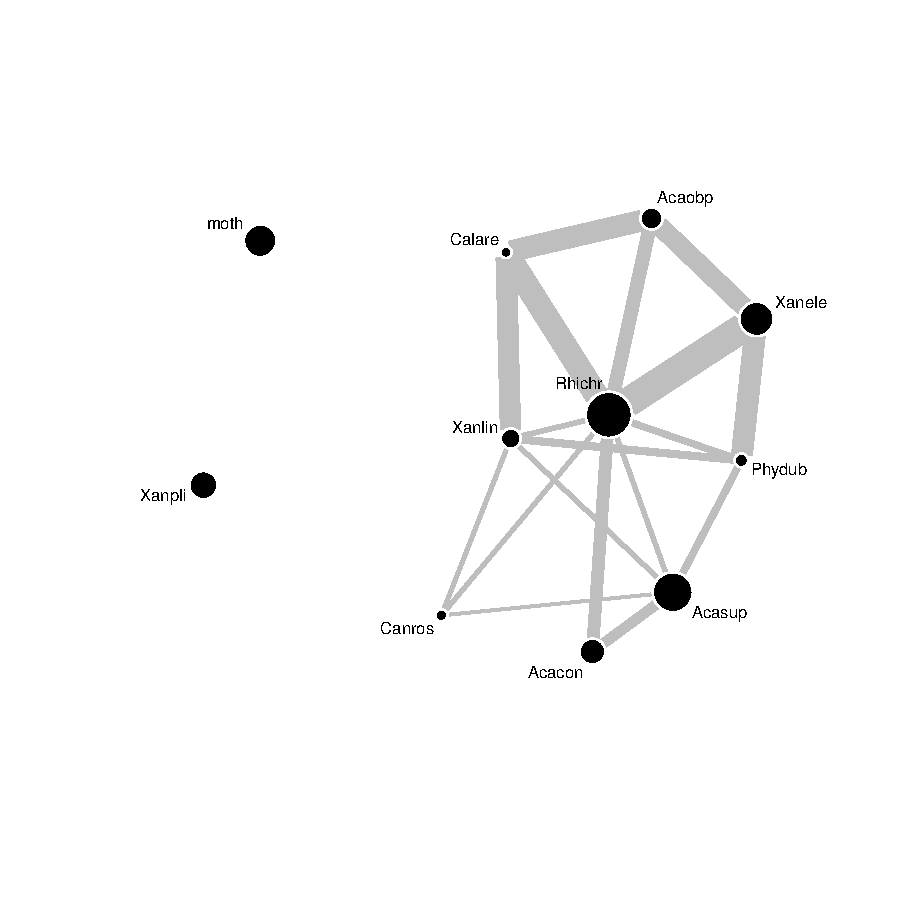
\includegraphics{SCRL-027}

%% %%Activate for bibtex vibliography
\bibliographystyle{plain}
\bibliography{/Users/Aeolus/Documents/bibtex/biblib}


\end{document}  


